%!TEX root = thesis.tex
\section{Data Steam Processing System Technology Overview}
\label{sec:overview}

This chapter describes the choices for data stream processing systems (DSPS) in which the pipeline for the Monash University
Institute of Railway Technology will be built, along with the methods which will be used for evaluating the different
technologies used. As identified in the the previous chapter, a number of relatively new DSPS technologies exist and have been in use
in different projects at different companies. Here we will look at more of an overview of the possibilities they offer
in terms of programming interfaces. Furthermore, we will outline the testing parameters that will be used in a later
chapter to evaluate the usage of each technology, highlighting both quantitative performance-based metrics as well as
qualitative metrics looking at the ease of programmability from the point-of-view of the DSPS programmer.

This chapter will first start with a look at the choices in DSPS technology which will be used further in the project,
in~\sectref{sub:dsps_technology_choices}, before going into the evaluation methods and approach in~\sectref{sub:evaluation_method_approach}.
Finally, we will look at an overview of the testing data in~\sectref{sub:overview_of_the_data}, before concluding in~\sectref{sub:conclusion}.


\subsection{Data Steam Processing System Technology Choices} % (fold)
\label{sub:dsps_technology_choices}

The DSPS technologies that have been chosen to be focused on in this sub-project include the following:

\begin{itemize}
  \item Samza
  \item Storm
  \item Spark Streaming
\end{itemize}

Literature concerning these DSPS technologies have been covered in~\sectref{sub:realtime_data_processing}, however
we will look into more depth into the systems regarding their usage from the programmer's point-of-view. Note that
in the previous chapter, a further DSPS technology, S4, was covered, however due to its notes decline in usage and
development in the chapter, it has been decided to omit the use of the technology from this project.


\subsubsection{Samza Programming} % (fold)
\label{ssub:samza_programming}

\textit{Note that most of the content in this section is sourced from the official Samza 0.9 documentation.}~\cite{Samza:doc}

Samza defines itself as a realtime data processing system which allows the processing of streams made up of immutable
messages of similar type or category. Streams in Samza exist independently of other concepts, allowing themselves to be
\textit{consumed} from or \textit{produced} to by various supported systems. The concepts of consuming and producing refer
to the actions of getting data from a stream and placing data onto a stream, respectively. Samza defines the systems that can be used
for consuming and producing to streams to be any piece of software that implements the stream abstraction. For example,
Kafka, a popular distributed messaging queueing system, is often used to consume and produce to Samza streams. Systems such as these can be
``plugged'' into a Samza project to work with the same streams which native Samza applications are written to work with.

For a Samza programmer, the most important concepts of the overall Samza project to understand are the concepts of the
\textbf{system} and \textbf{task}. In a Samza project, a system exists to produce a particular stream which then can
be processed by a task which consumes it. A task will always then produce output to another stream. Systems and tasks
can then be arranged in a pipeline-like structure allowing a specified type of processing on the messages which travel
on those streams. Hence, it is easy to think of a system as the source of data for an overall Samza project. A very
simple example of such a Samza project is shown in~\figref{fig:samza_overview}.

\begin{figure}[h]
  \centering
  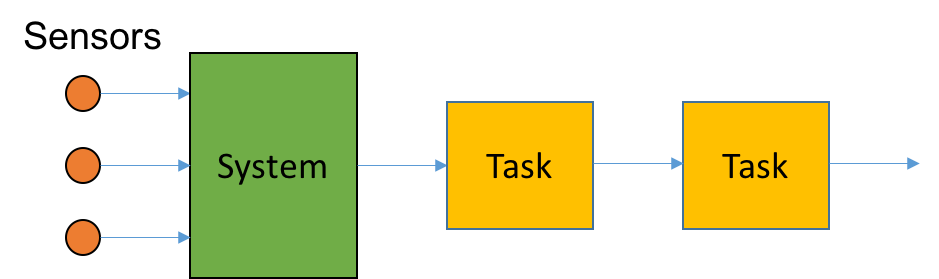
\includegraphics[width=0.8\textwidth]{includes/figures/fig_samza_overview}
  \caption{A simple Samza pipeline showing the roles of the system, task, and stream concepts. Streams are represented
  as arrows.}
  \label{fig:samza_overview}
\end{figure}

When programming a Samza project, interfaces exist for both the system and task concepts through the \texttt{org.apache.samza.system.SystemConsumer}
and \texttt{org.apache.samza.task.StreamTask} Java interfaces. Existing systems exist in the Samza project, and may be
used to produce streams which can then be processed by an implemented \texttt{StreamTask}.

The \texttt{StreamTask} interface is arguably the main interface in which the most important processing will be done in
a Samza project. It requires implementing a single method, \texttt{process}, which passes in an immutable message from the stream
on which the task is configured to consume. These messages are then processed as specified by the programmer before the
result of the processing is wrapped in a message envelope and produced to a stream specified by the programmer.

The streams on which \texttt{StreamTask} implementations consume are specified in a task specific configuration file,
independent to that of the implementation source code. These configuration files offer a range of parameters for the
execution of tasks, each of which are documented\footnote{https://samza.apache.org/learn/documentation/0.9/jobs/configuration-table.html},
however can result in quite verbose and hard to understand configurations files. For each task configuration, a system
needs to be defined that produces to the stream that the task consumes from. These can either be a self-implemented
system, or an existing pluggable system, such as Kafka.

For self-implementation of systems, then \texttt{SystemConsumer} interface requires much more understanding and effort to
implement than that of the \texttt{StreamTask} interface. Methods, such as \texttt{start}, \texttt{stop}, \texttt{register},
and \texttt{poll} need to be implemented, allowing for the producing of messages onto a particular stream. The \texttt{start}
and \texttt{stop} methods simply connect and disconnect the system to the underlying system, while the \texttt{poll}
method takes care of producing any messages from the system. The \texttt{register} method is much more complicated in the
way that it requires registering the implemented system with lower-level components of Samza to integrate the system into
Samza.

Note that, due to Samza's relative infancy to other DSPS technologies, many of these interfaces either completely lack
or offer insufficient documentation. Furthermore, for the same reason, example Samza projects are hard to find. This is
a key factor that will be touched upon in later chapters on evaluating the DSPS technologies.

Samza projects are generally compiled and distributed as JAR files, which may or may not contain project dependencies,
which then can be run directly on installed Samza distributions. Assembly of these JAR files are conventionally performed
through use of Java build automation tools, such as Maven or Gradle.

% subsubsection samza_programming (end)


\subsection{Storm Programming} % (fold)
\label{sub:storm_programming}

\textit{Note that most of the content in this section is sourced from the official Storm documentation.}~\cite{Storm:doc}

Storm defines itself as a distributed realtime computation system that provides primitives for performing realtime
computations. Storm compares itself to existing big data systems, such as Hadoop MapReduce, which similarly provides
primitives for performing batch data computations.

Like Samza, Storm also is built around the key concept of a stream, however Storm's definition of a stream slightly
differs to that of Samza's. In Storm, a stream is defined as an unbounded sequence of immutable tuples, rather than a sequence
of immutable messages as they are defined in Samza. A tuple is defined as a dynamically typed list of values, in which
the values can be of any type. Rather than consuming and producing to streams, Storm approaches computations on streams
through \textit{stream transformations} using the previously mentioned realtime computation primitives.

The realtime computation primitives that Storm offers are the components of Storm that are of most interest to the programmer.
These primitives are known as the \textbf{spout} and \textbf{bolt}, previously looked at in~\sectref{ssub:storm}. To compare
these components to those present in Samza, the spout acts as a source of streams, much like Samza's systems, while the
bolts acts as consumers of streams, which process and emit new streams, much like Samza's tasks. Storm offers interfaces
for implementation of custom spouts and bolts through the \texttt{backtype.storm.spout.ISpout} and \texttt{backtype.storm.task.IBolt}
interfaces, respectively.

As explained in~\sectref{ssub:storm}, spouts and bolts are arranged in a particular way to make up an overall Storm topology,
which is used to transform streams in some specified manner. A simple example of such a topology is shown in the previous
chapter, in~\figref{fig:storm_topology}.

Basic spouts require implementation of multiple methods, \texttt{open}, \texttt{nextTuple}, and \texttt{declareOutputFields},
which act as a spout initialiser, handler for each tuple to be emitted to a stream, and a tuple type declaration, respectively.
Implementation of a simple spout is a much easier task in Storm than a system in Samza, due to different provided interfaces
depending on the type of configuration needed for a particular spout. For example, a very basic spout can be made, using
a lot of default configuration options, by implementing the \texttt{backtype.storm.topology.base.BaseRichSpout} interface.

Bolts also require implementation of three main methods, \texttt{prepare}, \texttt{execute}, and \texttt{declareOutputFields},
allowing bolts to be initialised, process received tuples in a specified manner, and declare tuple value types, respectively.

One major point of different with this components, to their analogous components in Samza, is that the spout and bolt
implements are completely independent to the overall Storm topology layout. In Samza, systems and tasks require the output
streams to be hardcoded within their respective implementations, however Storm has a further separate source file for
defining the topology layout. This topology layout is generally defined in a separate file to all spout and bolt implementations
using the provided \texttt{backtype.storm.topology.ToplogyBuilder} class. This class exposes methods for defining the
topology layout, in terms of spout and bolt placement, along with inputs and outputs for each spout and bolt implementation,
as well as overall topology configuration. An obvious downside to this over Samza configuration files is that it requires
a recompilation in the case that configuration options need to be tweaked, while Samza configuration files are not part
of the compiled source code.

Storm topologies are generally compiled and distributed in the same way as Samza projects; as JAR files containing compiled
bytecode, assembled using Java build automation tools.

% subsection storm_programming (end)


\subsection{Spark Streaming Programming} % (fold)
\label{sub:spark_streaming_programming}

\textit{Note that most of the content in this section is sourced from the official Spark Streaming 1.3.1 documentation.}~\cite{Spark:doc}

While many analogies can be made between the key components of Storm and Samza, due to their similarities in design and
usage, Spark Streaming presents itself differently. Spark Streaming defines itself as an extension of its parent project,
Spark, a big data batch processing system, which affords scalable, high-throughput, fault-tolerant stream processing of
live data streams. Data can be streamed into Spark Streaming using a variety of supported sources, from complicated data
systems, such as Kafka, to low-level sources, such as TCP sockets.

Internally, Spark Streaming processes data quite differently to Samza and Storm, due to being an extension to the base
Spark batch processing system. Data streams are fed into Spark Streaming, which automatically partitions the streams into
small batches which are then sent to the underlying Spark batch processing engine. The Spark batch processing engine then
outputs a stream of results made up of multiple batches of data. A diagram illustrating this process is shown in~\figref{fig:spark_stream_batch}.

This way of processing streams as a sequence of batches is all enabled through Spark Streaming's stream abstraction,
discretised streams, or DStreams. It differs to how streams are conceptualised in Samza and Storm in the way that while
streams are still, in essence, an unbounded sequence of data structures, being tuples in Storm, and message envelopes in
Samza, these data structures are the same data structure which is used to represented data batches in Spark. These are,
of course, the same resilient distributed dataset (RDD) data structure as explained in the previous chapter, in~\sectref{ssub:spark_streaming}.
Hence, Spark Streaming DStreams can be decomposed into a sequence of RDDs, making them fully compatible with batch-mode Spark.

For programming a Spark Streaming job, there are not a set of provided interfaces expected to be implemented, like in
Samza or Storm. Instead, all of the computations to be performed on streams are performed on an instantiation of the
\texttt{org.apache.spark.streaming.dstream.DStream} class returned from a DStream producing function from the
\texttt{org.apache.spark.streaming.StreamingContext} class. Processing performed on DStreams are generally programmed in
a dataflow fashion, with each function performed on the DStream returning a new DStream.

This way of operating on DStreams in a Spark Streaming program leads to all processing being contained in a single file,
whereas in Storm or Samza processing would be split between tasks or bolts written in different files. This leads to
more straightforward control over DStream transformations when programming, however also leads to much more tightly
coupled logic. This will be a topic of interest later when evaluating the different DSPS technologies.

Spark Streaming programs are compiled and distributed in the same fashion in which Samza and Storm projects are. However,
for Spark Streaming programs written in Python using their relatively new PySpark API, compilation is unnecessary and an entire Spark
Streaming Python project can be distributed and submitted and run on different installations of Spark Streaming straight
from the Python source file. This greatly eases the distribution and deployment aspects of Spark Streaming, when using
PySpark, in relation to Storm topologies and Samza projects.

% subsection spark_streaming_programming (end)

% subsection dsps_technology_choices (end)



\subsection{Evaluation Method \& Approach} % (fold)
\label{sub:evaluation_method_approach}

Evaluation of each of the chosen DSPS technologies will be performed using both qualitative and quantitative testing methods
of evaluation. The quantitative evaluation methods used will focus
on the benchmarking of various features that are common to each of the technologies, and the comparison of the features that
each technology supports. The qualitative evaluation methods will focus on looking at the differences in ease-of-use,
support for different programming languages and features, and complexity of code written to implement the pipeline on
each of the different DSPS technologies.

With looking at the decision of giving a clear recommendation for a particular technology out of the choices stated,
we think it is import to look at both qualitative and quantitative aspects for comparison. These systems are significantly
non-trivial and vastly different in design and usage. However, as they still afford the same possible functionality,
it is very possible to give a properly constructed evaluation of them. Not only is a factor such as performance a critical
factor in forming a recommendation, but also are the possibilities each technology affords, in terms of programming and
extensibility, when recommending a technology for use in such a large, and long production-life project.


\subsubsection{Quantitative methods} % (fold)
\label{ssub:quantitative_methods}

The quantitative methods to be used to evaluate the candidate DSPS technologies include mostly performance-based
metrics. Each of the metrics that will be used is as follows:

\begin{itemize}
  \item DSPS start-up time
  \item Response time to single data value
  \item Throughput time for large amounts of streamed data
  \item System resource usage
  \item Available DSPS features
\end{itemize}

DSPS start-up time refers to the amount of time between submitting a ready job to a DSPS technology to the time when
the system is at a ready state to begin processing incoming data streams. We consider this to be a less important performance
metric to assess, however it is still of interest to see the differences present in each candidate technology. It is less
important as, for the most part, it will not affect overall performance of each processing system as they will generally
be running at all times, waiting for data to be streamed in. This metric will be consistently measured using the internal
logs for each DSPS technology.

Response time to a single data value refers to the amount of time taken for each given DSPS technology to completely
process a given value sent onto the processing stream through the entire implemented pipeline. The same data value of
``42'' will be sent onto the stream, and we will be expecting a result of \texttt{(42, true)}. This result will be
further explained in the next chapter as we look at the design and implementation of the processing pipeline and simple
task it will need to perform. Response time to a single data value is quite an important performance metric to consider
as in the real use of the pipeline, as, most of the time, single data values, representing sensor readings, will be placed
onto the respective DSPS technology's processing pipeline. The speed at which each technology can process these data
values is important to the overall performance of the system as it will enable more data to be processed without forcing
large queues of pending data.

Throughput time for large amounts of streamed data refers to the amount of time taken to process large batches of data
delivered at once. While this is less of a realistic use-case for testing in relation to the Monash IRT project, as data
is not expected to be delivered in such large amounts, it is aimed at looking to stress-test each of the candidate DSPS
technologies to see how they perform and scale to deal with different high-stress data loads. For this stress-test, we
will look at five different ranks of tests, using data sets containing 100,\@000, 500,\@000, 1,\@000,\@000, 5,\@000,\@000, and
10,\@000,\@000 data values. These data sets will be generated using sample data, received from the Monash IRT team, of
prior sensor readings in the IRT project. Throughput time will be measured from the time processing begins on the incoming
data, to the time in which all data values in the datasets have finished being processed.

System resource usage refers to the peak amount of resident system memory that is being used by each of the candidate DSPS
technologies during processing. We are to measure the peak resident memory usage as this gives an accurate overall indication of
how stressful each DSPS technology is to host the operating system. Other system resource metrics, such as CPU usage, have
been omitted from tests as each system uses all available CPU processing power to process its data. Resident memory usage
will be measured using the built-in UNIX \texttt{ps} system utility\footnote{http://unixhelp.ed.ac.uk/CGI/man-cgi?ps}.

Available DSPS features refers to the features each candidate DSPS technology supports as they relate to Stonebraker,
\c{C}\~entintemel, and Zdonik's eight requirements for realtime data processing systems, as looked at in the previous
chapter in~\sectref{sub:processing_conclusion}. The supported features for each technology will be compared to show the
processing possibilities available in each technology.

% subsubsection quantitative_methods (end)


\subsubsection{Qualitative methods} % (fold)
\label{ssub:qualitative_methods}

The qualitative methods used to evaluate the candidate DSPS systems include mostly programmer-centric metrics, showing the
programming possibilities for each technology. Each of the metrics that will be compared is as follows:

\begin{itemize}
  \item Ease of programmability
  \item Ease of deployment
  \item Ease of pipeline extensibility
\end{itemize}

Ease of programmability refers to a number of different features including official programming language support, complexity
of required interfaces to be implemented, and complexity of required system configuration. To summarise, we will look at
the difficulty and learning-curve that may need to be overcome to program each candidate DSPS technology. Measuring this
presents a more difficult, and somewhat subjective, task compared to the metrics used in the quantitative metrics, however
these will be measured using impartial comparisons of the methods which each technology affords to be programmed.

Ease of deployment refers to the methods each candidate technology affords its projects to be deployed and distributed.
Similar to with ease of programmability, this metric will be measured by an impartial comparison of each possible
method of project deployment and distribution.

Ease of pipeline extensibility refers to the methods used to extend an existing pipeline, or project, existing in each
of the candidate technologies. For example, if an existing project is already in production, we will be measuring the
ease of which each technology allows that project to be extended in the ways of adding further processing tasks to the
existing system, or restructuring an existing project processing layout (for example, a Storm topology layout). Parameters
we will be looking at include whether or not an entire project needs to be recompiled and deployed to be extended, and the
ease of modifying overall system configurations.

% subsubsection qualitative_methods (end)

% subsection evaluation_method_approach (end)


\subsection{Overview of the data} % (fold)
\label{sub:overview_of_the_data}

As this sub-project focuses on the realtime processing of streaming data, data streams will have to be simulated from
datasets acquired from the Monash IRT team. An initial dataset has been given that consists of sensor data in the
categories as shown in~\tabref{tab:irt_data}.

\import{includes/tables/}{data_table}

The sample data acquired from the IRT team includes 99\,999 rows of data recorded from each of the shown sensors,
organised in a CSV file with headers. This is a general example of how data is currently received and handled by the IRT
team, however in the case of realtime data processing, data would be received in quite a different manner. Rather than
being received in large batches of readings, such as the sample dataset acquired, streams of data may be created from
each particular sensor, delivering data values to the DSPS systems along input streams a single value at a time. Data
is streamed in an asynchronous fashion, and can be simply thought of as a given DSPS system listens on an incoming stream, and
acts upon any data value in a specified fashion whenever they may be received.

Hence, to simulate streaming data from the data samples we have acquired, the DSPS pipeline is constructed to listen on
a particular TCP socket connection for any incoming data. Once a data value is encountered on the connection, it is fed into
the pipeline and processed accordingly while the pipeline continues to listen on the socket for further incoming data.
As the pipeline is constructed in such a way, we can simulate the data being sent out from sensors using a program such
as \texttt{netcat}\footnote{http://nc110.sourceforge.net/}, where we can pipe data from a file to a particular
socket over a connection. We can also have time intervals between each data value, simulating time between sensor readings.

For the test data for the quantitative tests, as each sensor's data reading values are of the same format (a floating point
number), the specific sensor data to be used in the tests is not of major concern. Instead, we have chosen to focus on
generating data based of the values from the speed sensor. As specified in~\tabref{tab:irt_data}, each value represents
a speed reading formatted in kilometres per hour as a floating point number. To generate the different datasets for the
data batches for the throughput time quantitative test, we have extracted the speed readings from the provided sample dataset
and replicated them a number of times to generate the large batches. Finally, this leaves us with five datasets containing
speed readings of sizes 100,\@000, 500,\@000, 1,\@000,\@000, 5,\@000,\@000, and 10,\@000,\@000 data values, respectively.

% subsection overview_of_the_data (end)


\subsection{Conclusion} % (fold)
\label{sub:conclusion}

In conclusion, we have examined the three chosen candidate DSPS technologies in detail in terms of the possibilities they
afford for the programmer, outlined the testing parameters which will be used in the overall evaluation of candidate
technologies, and the data in which will be used in the highlighted tests. These components lay down a framework for
implementation and testing which will be looked at in the following two chapters, respectively.


% subsection conclusion (end)
